% !TEX encoding = IsoLatin
\documentclass[12pt, a4paper]{article}
\usepackage[utf8]{inputenc}
\usepackage[T1]{fontenc}
%\usepackage[latin1]{inputenc}
\usepackage[hmargin = 25mm, vmargin = 25mm]{geometry}
%\geometry{letterpaper}                   % ... or a4paper or a5paper or ... 
%\geometry{landscape}                % Activate for for rotated page geometry
%\usepackage[parfill]{parskip}    % Activate to begin paragraphs with an empty line rather than an indent
\usepackage{graphicx}
\usepackage{amssymb, amsmath, amsthm}
\usepackage{epstopdf}
\usepackage{moreverb}
\usepackage{hyperref}
\usepackage{algorithm,algorithmic}
\usepackage[french]{babel}
\usepackage{hyperref}
\usepackage{fancyhdr} 
\usepackage{float}
\pagestyle{fancy}

\renewcommand{\headrulewidth}{0pt}
\fancyhead[C]{} 
\fancyhead[L]{}
\fancyhead[R]{}

\renewcommand{\footrulewidth}{0pt}
\fancyfoot[C]{\footnotesize{$13^{es}$ Journées de méthodologie statistique de l’Insee (JMS) / 12-14 juin 2018 / PARIS}}
\fancyfoot[R]{\thepage}

\begin{document}

\begin{center}

\includegraphics[width=15cm]{head_jms2018.png} 
\line(1,0){450}
\vspace{5mm}
\textbf{{\huge \'E}\Large LABORATION D'UNE MAILLE GEOGRAPHIQUE POUR L'HABITAT}
\end{center}

\begin{center}
\textit{Solène COLIN(*), Vivien ROUSSEZ(*)} \\
%- N. B. le premier nom doit être celui de l'auteur qui effectuera la présentation orale (sauf contributions associées)
\vspace{2mm}
\textit{(*) CGDD, Service de la Donnée et des \'Etudes Statistiques}\\ 

\vspace{2mm}
\url{solene-c.colin@developpement-durable.gouv.fr} \url{vivien.roussez@developpement-durable.gouv.fr} 
\end{center}
\vspace{5mm}
\small{{\bf Mots-cl\'es.} Analyse spatiale, graph mining, clustering, analyse multidimensionnelle, cartographie.}

\begin{center}
\line(1,0){450}
\end{center}


\section*{Résumé}

Le SDES a lancé en 2017 un projet visant à construire un maillage du territoire à même de rendre compte des disparités territoriales sur les enjeux propres au logement. En effet, ni les échelles administratives, ni les zonages d'études de l'Insee (zones d'emploi, bassins de vie) ne sont adaptées pour l'analyse localisée du logement, car ils mêlent dans les mêmes mailles des types d'habitat différents (urbain et périurbains notamment). Pour cela, neuf indicateurs représentatifs de l'équilibre des marchés du logement ont été sélectionné pour alimenter la méthode de \textbf{régionalisation}, qui regroupe les communes en bassins homogènes. La méthode retenue est l'algorithme \textbf{SKATER} (Spatial Klustering Analysis by Tree Edge Removal), qui s'appuie sur l'exploration de graphe et notamment la notion d'arbre portant minimal. \\

Différentes simulations ont été menées pour déterminer la taille de ces mailles, et les résultats ont fait l'objet de tests au niveau régional. Ces mailles mettent au premier plan les disparités propres au logement (pouvoir d'achat immobilier, taille des ménages), alors que la maille communale fait principalement ressortir les disparités liées au degré d'urbanité. Elle permet également de distinguer les villes-centre de leur périphérie, et donc d'isoler les enjeux propres à ces espaces très différents sur le plan du logement. \\

L'analyse de ces mailles permet de mettre en exergue six types de marchés locaux du logement, principalement distingués par le niveau des prix, la composition des ménages (leur taille) et du parc de logement. Au fil du temps, les spécificités de ces marchés se renforcent et ceux déjà en tension voient leurs déséquilibres se renforcer. A l'inverse, le ralentissement démographique et le vieillissement à l'\oe uvre dans les espaces faiblement peuplés contribuent à la faible dynamique des marchés où la demande est déjà modérée. Par ailleurs, ces marchés présentent un degré inégal d'homogénéité, et on trouve d'avantage de diversité entre les communes de marchés de l'Est de la France.

\section*{Abstract}

Partant du constat que les mailles géographiques usuelles ne permettent pas une analyse fine des marchés du logement, le SDES a élaboré une maille ad hoc. Pour cela, 9 indicateurs emblématiques de la demande et de l'offre des marchés locaux du logement ont été sélectionnés et ont alimenté une méthode de \textbf{régionalisation} utilisant la théorie des graphes et les arbres portants minimaux. Ce maillage permet une lecture facilitée des dynamiques territoriales sur les plans du logement et de la démographie.


\section*{Introduction}

Les mailles habitat constuites par le SDES ont pour objectif de constituer une échelle pertinente pour l'observation et l'analyse des enjeux territoriaux liés à l'habitat. Elle permet de répondre à trois objectifs :

\begin{itemize}
\item Lisser visuellement l'information pour donner des cartes lisibles
\item Conserver au maximum les disparités territoriales, tout en faisant ressortir les enjeux propres à l'habitat
\item Alimenter la connaissance et les diagnostics locaux
\end{itemize}


Pour cela, le SDES a construit des ensembles de communes qui \emph{se ressemblent} sur le domaine de l'habitat. Cette approche diffère de celle de l'Insee qui, pour ses zonages d'études, regroupe les communes qui sont fortement connectées les unes aux autres. Ce degré de connexion s'apprécie à l'aune du nombre de navettes domicile-travail entre les communes (pour les zones d'emploi) et les flux (théoriques) d'habitant se déplaçant de leur commune de résidence vers le pôle de services le plus proche (pour les bassins de vie). Pour plus d'information sur les maillages produits par l'Insee, consultez \href{https://www.insee.fr/fr/information/2114631}{cette page}.

\section{Sélectionner les indicateurs pertinents}

Choisis dans le cadre de deux comités regroupant des experts des territoires et du logement, les 9 indicateurs mobilisés sont représentatifs des marchés du logement, à la fois dans l'offre, la demande, et les équilibres de marché.

\subsection{Quels indicateurs}

Ces indicateurs sont calculés à partir de trois sources : recensements de la population, Filocom (Fichier des Logements localisés à la Commune), bases notariales (PERVAL et BIEN). Certaines communes ne présentant pas de donnée pour un ou plusieurs indicateurs, une \textbf{imputation} a été réalisée en prenant (de façon spatialement récursive) la moyenne de cet indicateur sur les communes voisines. Ces indicateurs sont présentés en détail dans le rapport méthodologique disponible sur le site internet du SDES.

\begin{enumerate}
\item L'indicateur de jeunesse du parc : part des logement récents (construits après 1975) rapportés à la part des logements anciens (construits avant 1949). 
\item Durée d'occupation médiane des logements
\item Taux de transactions dans le marché de l'ancien (nombre de transactions rapporté au nombre de logements)
\item Part de logements sociaux
\item Part de logements en situation de suroccupation
\item Prix au $m^2$ dans l'ancien rapportés au revenu médian communal
\item Nombre de personnes par ménage
\item Part des résidences secondaires
\item Part de logements vacants
\end{enumerate}


\subsection{Analyse de quelques indicateurs}

\subsection{Validation des indicateurs}

\subsubsection{Analyse en composantes principales}

Pour valider le choix des indicateurs sélectionnés (plusieurs itérations ont été nécessaires), une analyse en composantes principales (ACP) a été réalisée sur la base des indicateurs retenus. L'objectif consistait à retenir un minimum d'indicateurs pertinents et surtout \textbf{non redondants}, mais en conservant également quelques mesures "incontournables" de l'état du marché du logement (la part de logements sociaux, notamment).

\begin{center}
\begin{figure}[H]
\caption{ACP sur les indicateurs retenus}
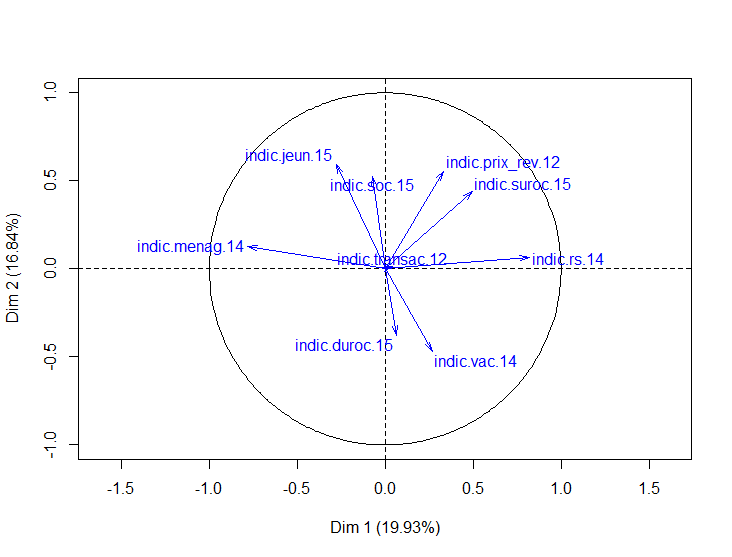
\includegraphics[scale=.7]{img/ACP.png}
\end{figure}
\end{center}

Les résultats de l'ACP montrent que les indicateurs ne présentent pas de redondance d'information, ce qui aurait pu conduire à sur-pondérer une dimension (le clivage urbain / rural par exemple). Les 6 axes retenus permettent de mettre en lumière un certain nombre de caractéristiques territoriales, résumées dans le tableau suivant : \\

\begin{figure}[H]
\caption{Principaux axes factoriels}
\begin{tabular}{| l | l | c | l |}
\hline
Axe factoriel & Variables constitutives       & Signe &  Disparités territoriales révélées \\
\hline
Axe 1         &Jeunesse du parc               & +    & Gradient urbain \\
              &  Taille des ménages             & +  &    \\
\hline
Axe 2         &Prix                           & +    & Gradient de tension \\
       & Suroccupation                  & +    & \\ 
      &Taille des ménages             & -  &   \\
\hline
Axe 3         &Vacance                        & -    & Zones touristiques \\
        &Logements sociaux              & -    &  \\
        &Durée d'occupation             & +    & \\
\hline
Axe 4         &Taux de transactions           & +    & Coeurs des AU  \\
                                           &  & & Marchés dynamiques de l'Ouest et du Nord \\
\hline
Axe 5         &Durée d'occupation             & +    & Zones Nord-Est (propriétaires) \\
        &Social                         & +    & versus Sud et Sud-Est \\
\hline
Axe 6         & Suroccupation                  & +    & Couronnes périurbaines et \\
                 & &                &  zones touristiques du Sud-Est \\
\hline
\end{tabular}
\end{figure} 

\vspace{.2cm}


\subsubsection{Classification communale}


Par la suite, on effectue une classification des communes par centres mobiles, opérée sur les coordonnées factorielles des 6 premiers axes. Cette classification permet de mettre en exergues six groupes de communes qui permettent de rendre compte des principales disparités territoriales attendues. 

\begin{center}
\begin{figure}[H]
\caption{Classification des communes}
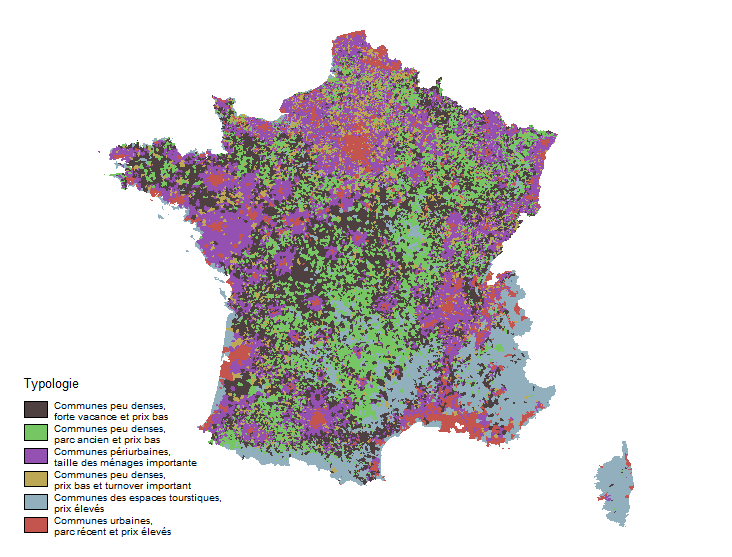
\includegraphics[scale=.7]{img/Typo_com.png}
\end{figure}
\end{center}

Ces types sont cohérents avec d'autres études déjà réalisées, soit sur la dimension territoriale, soit sur  le logement. Ils confirment le choix des indicateurs qui a été fait. C'est donc sur cette base qu'est faite la régionalisation.


\section{La régionalisation}

La \textbf{régionalisation} désigne l'opération qui consiste à regrouper des unités géographiques élémentaires en un ensemble \textbf{contigu}, selon des critères statistiques. Il existe un grand nombre de méthodes de régionalisation, dont une partie est comparée dans \href{http://journals.sagepub.com/doi/pdf/10.1177/0160017607301605}{cet article}. Le SDES a retenu l'algorithme SKATER (Spatial Klustering Analysis by Tree Edge Removal), implémenté et mis à disposition dans le package \textsc{spdep} du logiciel statistique libre\textsc{R}.

\subsection{L'algorithme SKATER}

Cet algorithme fonctionne en 4 étapes :

\begin{enumerate}
\item Construction de la matrice de contiguïté $\rightarrow$ obtention d'un \emph{graphe} (un noeud = une commune et un lien = relation de contiguïté entre deux communes)
\item Pondération de ce graphe avec les dissimilarités calculées à partir des indicateurs (distance euclidienne)
\item Construction de l'\textbf{arbre} portant minimal, en retenant le lien avec le voisin le plus ressemblant pour chaque n\oe ud du graphe
\item Suppression itérative des branches de l'arbre maximisant la variance inter-classes des sous-graphes obtenus après élagage.
\end{enumerate}

Il peut donc être vu comme une forme de classification descendante hiérarchique opérée sur les liens de l'arbre portant minimal. Le fait de travailler à partir de cet arbre portant minimal plutôt que sur les n\oe uds du graphe garantit la contiguïté des mailles finales.

\begin{center}
\begin{figure}[H]
\caption{Illustration des étapes de SKATER sur les Hauts de Seine}
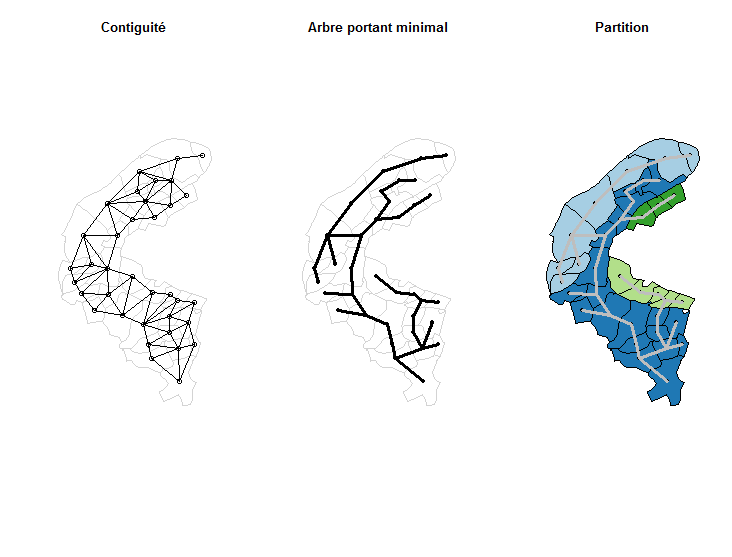
\includegraphics[scale=.7]{img/SKATER.png}
\end{figure}
\end{center}

\subsection{Découper le problème}

Cet algorithme est très couteux : sa complexité est en effet légèrement supérieure à $o(n^2)$, et il n'a pas été optimisé dans un langage plus efficace que R. En conséquence, il est impossible de traiter les près de 36000 communes françaises. En effet, le traitement de l'Île-de-France (moins de 1300 communes) prend environ 5 minutes, alors qu'il faut 3 heures pour le Grand-Est (environ 5000 communes). C'est pourquoi l'algorithme a été exécuté région par région. Toutefois, pour s'affranchir de ces limites administratives, on procède à un \emph{lissage} des frontières régionales. Pour cela, on identifie les zones qui touchent une frontière régionale et on refait un zonage à partir de l'ensemble des communes qui en font partie.\\
L'ordre de grandeur du nombre de communes qui se trouvent dans les zones concernées est de 16 000. La difficulté liée au temps de calcul apparaît donc de nouveau. Pour contourner ce problème, il faut couper cet ensemble en plusieurs sous-ensembles de taille plus petite. Pour réaliser ce découpage, on a repéré le barycentre du pays. La zone se trouvant sur ce barycentre, ainsi que les zones contiguës constituent une première \emph{macro-zone}.


\begin{center}
\begin{figure}[H]
\caption{Répartition des zones frontalières}
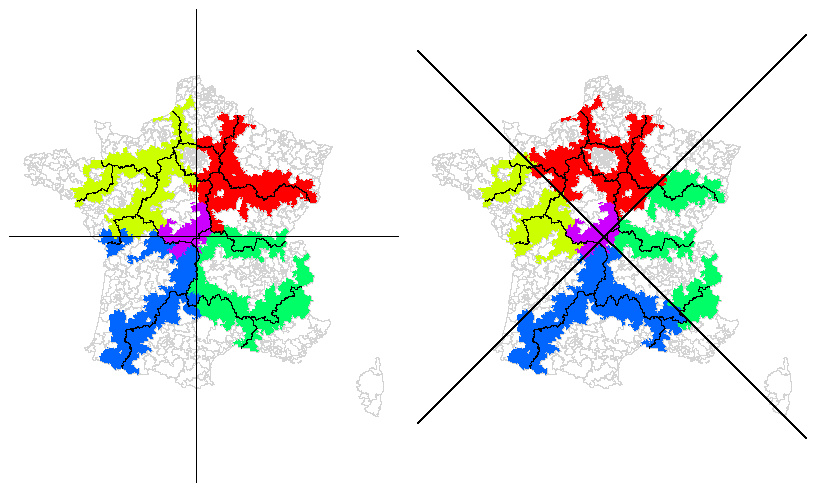
\includegraphics[scale=.7]{img/Methodo_decoupage.png}
\end{figure}
\end{center}


On répartit ensuite le reste des communes dans les 4 cadrans du repère orthonormé ayant pour origine ce barycentre. Toutefois, les axes de ce repère passant le long de frontières, on conserve en partie l'effet de frontière. Pour éviter se biais, on effectue une rotation du repère orthonormé de 45 degrés.
Cette méthode fait néanmoins apparaître, selon les cas de figure, de très petites zones isolées, et des macro-zones qui ne sont pas contigües. Une dernière étape consiste donc à rattacher les isolats à la macro-zone contiguë de taille suffisante ou à séparer les parties non contiguës des grandes macro-zones.

\begin{center}
\begin{figure}[H]
\caption{Découpage final en macro-zones}
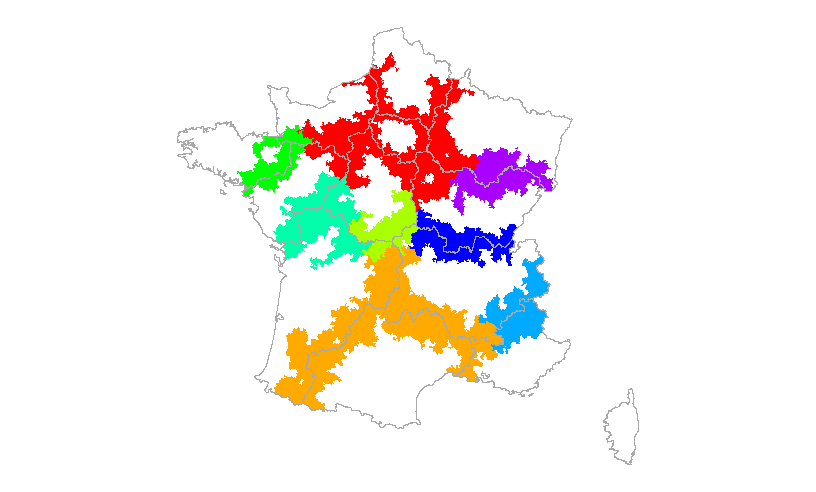
\includegraphics[scale=.7]{img/Decoupage.png}
\end{figure}
\end{center}

\subsection{Les différentes simulations}

L'algorithme fonctionne à l'aide de deux paramètres qui permettent de faire varier le résultat final : le nombre de mailles finales souhaitées et une taille minimale (en termes de nombre de communes, de population, de nombre de logements...). 

\section{Caractérisation des mailles}

\subsection{L'habitat au premier plan}

\subsection{Typologie des mailles}

\subsection{Cohésion et dynamique de ces mailles}

\nocite{*}
%\bibliographystyle{acm}
%\bibliography{DB}

\end{document}  